\subsubsection{Overview}

The B-Tree can be regarded as a function $\mathcal{F}$ that maps the key $x$ into its corresponding page index $y$. It is known to us that the pages are allocated in a way that the every $S$ entries are allocated in a page where $S$ is a pre-defined parameter. For example, if we set $S$ to be 10 items per page, then the first page will contain the first 10 keys and their corresponding values. Similarly, the second 10 keys and their corresponding values will be allocated to the second page.

If we know the CDF of $X$ as $F(X\leq x)$ and the total number of entries $N$, then the position of $x$ can be estimated as $p=F(x)*N$ and the page index where it should be allocated to is given by

$$y=\floor{\frac{p}{S}}=\floor{\frac{F(x)*N}{S}}$$  

\begin{mscexample}

For example, if the keys are uniformly distributed from $0$ to $1000$, i.e. the CDF of $X$ is defined as $F(X\leq x)=\frac{x}{1000}$ and we set $S=10, N=1001$. Then for any key $x$, we immediately know it will be allocated into $y=\floor{\frac{1000}{10}*\frac{x}{1000}}=\floor{\frac{x}{10}}$. Assume that we have a key $698$, then we can calculate $y=\floor{\frac{698}{10}}=69$. By doing so, the page index is calculated in constant time and space.

\end{mscexample}



In this example, we see that the distribution of $X$ is essential and our goal of learned index in one-dimensional data is to learn such distribution. To do so, we apply two different techniques as the baseline, the polynomial regression and fully connected neural network.

To train such a learned index, we first manually generate the $X$ with respect to a certain distribution. We then save the generated $X$ into a dense array with the length $N$. Then we use the proportional index, i.e. the index of each $x$ divided by $N$ as the expected output $y$.
 
\subsubsection{Fully Connected Neural Network}

After generating the training dataset $X$ and its corresponding $Y$, we build a fully connected neural network as the baseline learned index. The architecture of the fully connected neural network is illustrated in Figure \ref{fig:baseline_fcn}.

\tikzset{%
  every neuron/.style={
    circle,
    draw,
    minimum size=1cm
  },
  neuron missing/.style={
    draw=none, 
    scale=4,
    text height=0.333cm,
    execute at begin node=\color{black}$\vdots$
  },
}
\begin{figure}
\center
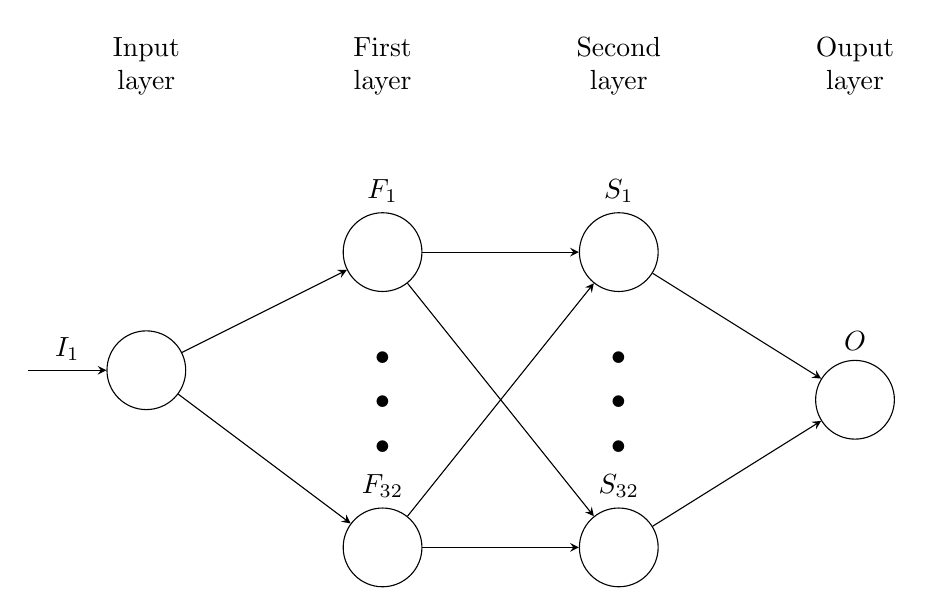
\begin{tikzpicture}[x=1.5cm, y=1.5cm, >=stealth]
\foreach \m/\l [count=\y] in {1}
  \node [every neuron/.try, neuron \m/.try] (input-\m) at (0,2.5-\y*2.75) {};

\foreach \m [count=\y] in {1,missing,2}
  \node [every neuron/.try, neuron \m/.try ] (first-\m) at (2,2-\y*1.25) {};

\foreach \m [count=\y] in {1,missing,2}
  \node [every neuron/.try, neuron \m/.try ] (second-\m) at (4,2-\y*1.25) {};

\foreach \m [count=\y] in {1}
  \node [every neuron/.try, neuron \m/.try ] (output-\m) at (6,1.5-\y*2) {};


\foreach \l [count=\i] in {1}
  \draw [<-] (input-\i) -- ++(-1,0)
    node [above, midway] {$I_{\l}$};

\foreach \l [count=\i] in {1,32}
  \node [above] at (first-\i.north) {$F_{\l}$};

\foreach \l [count=\i] in {1,32}
   \node [above] at (second-\i.north) {$S_{\l}$};

\foreach \l [count=\i] in {1}
   \node [above] at (output-\i.north) {$O$};

\foreach \i in {1}
  \foreach \j in {1,...,2}
    \draw [->] (input-\i) -- (first-\j);

\foreach \i in {1,...,2}
  \foreach \j in {1,...,2}
    \draw [->] (first-\i) -- (second-\j);

\foreach \i in {1,...,2}
  \foreach \j in {1}
    \draw [->] (second-\i) -- (output-\j);

\foreach \l [count=\x from 0] in {Input, First, Second, Ouput}
  \node [align=center, above] at (\x*2,2) {\l \\ layer};

\end{tikzpicture}
\caption{The architecture of the fully connected neural network used as baseline learned index. In this neural network, we use only 2 fully connected layers and each layer is equipped with 32 neurons. The input of this neural network is only one neuron such that it represents the given query key. The output of this neural network is limited to 1 neuron such that it represents the predicted proportional position of the key value pair.}
\label{fig:baseline_fcn}
\end{figure}

We apply Rectified Linear Unit (ReLU) activation function at the end of $F_i$ and $S_i$. Formally, assume the output of $F_i$ is $a$, then we define the output of $F_i$ as $y=max\{a, 0\}$. Then we train this fully connected neural network with standard stochastic gradient descent (SGD), and we set the learning rate to be $lr=0.001$. 

Formally, we can induce the output of this fully connected neural network as following:

